\chapter{Oxidation and Reduction in Organic Chemistry}\label{ch:b1:organic-redox}

A bottle of wine left open turns, within days, into vinegar: bacteria use
the oxygen of the air to oxidise ethanol into ethanoic acid. A ketone and
the alcohol it comes from differ by two hydrogen atoms --- and, counted
properly, by two electrons. Organic oxidations and reductions do not look
like the exchanges of electrons between metal ions of \cref{ch:b1:nernst},
because electrons travel with protons or with hydride ions, but the
bookkeeping is the same. This chapter assigns \omterm{def:b1:organic-redox:oxidation-level}{oxidation levels} to carbon,
uses them to predict what each alcohol gives when oxidised, and
introduces the hydride reagents that reduce carbonyl compounds, with an
eye on which groups each reagent leaves untouched.

\begin{recall}
\omterm{def:b1:nernst:oxidation-number}{Oxidation numbers}, \omterm{def:b1:nernst:couple}{half-equations} and the balancing of redox equations are
in \cref{ch:b1:nernst}; the classes of alcohols and of carbons in
\cref{ch:b1:electronic-effects}; \omterm{def:b1:acetals-protection:hemiacetal}{acetals} and the \omterm{def:b1:acetals-protection:protecting-group}{protection} of carbonyl
groups in \cref{ch:b1:acetals-protection}; Grignard additions in
\cref{ch:b1:organomagnesium}.
\end{recall}

\begin{omfigure}
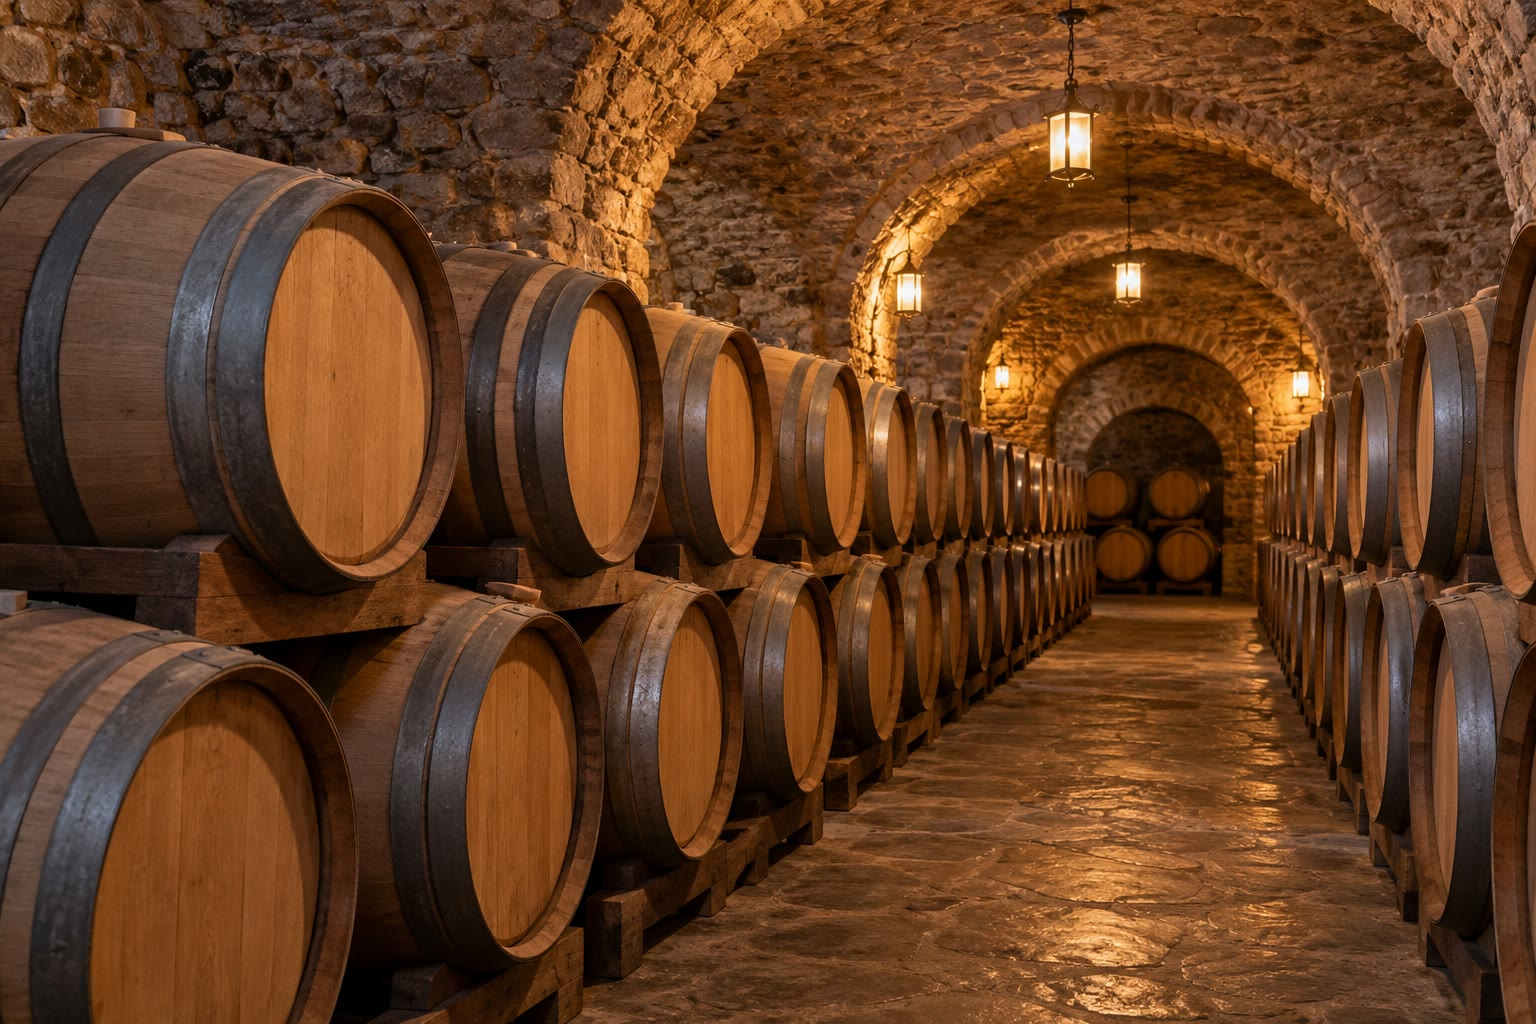
\includegraphics[width=0.58\linewidth]{images/book2/ai/b1-24-wine-cellar.jpg}

{\small Wine aging in a cellar. Kept from air, wine keeps its ethanol;
exposed to air, acetic acid bacteria oxidise it to ethanoic acid.}
\end{omfigure}

\section{Oxidation levels of carbon}

\begin{definition}[Oxidation level]\label{def:b1:organic-redox:oxidation-level}
The \emph{oxidation level}\index{oxidation level} of a carbon atom is its
\omterm{def:b1:nernst:oxidation-number}{oxidation number}, obtained by the rules of
\cref{prop:b1:nernst:on-rules}: each bond to a more electronegative atom
(O, N, halogen) counts $+1$, each bond to hydrogen $-1$, each bond to
another carbon 0 (a double bond counts twice).
\end{definition}

\begin{proposition}[Oxidation numbers of carbon]\label{prop:b1:organic-redox:on-of-carbon}
The \omterm{def:b1:nernst:oxidation-number}{oxidation number} of a carbon equals (number of bonds to O, N or
halogens) minus (number of bonds to H). Within one family of compounds
of the same carbon skeleton, alcohol $\to$ aldehyde or ketone $\to$
carboxylic acid $\to$ carbon dioxide is a series of oxidations by two
electrons each.
\end{proposition}

\begin{proof}
Breaking every bond and giving both electrons to the more electronegative
partner: from H (less electronegative than C) carbon gains an electron,
charge $-1$ per C--H; to O, N, halogens (more electronegative) it loses
one, $+1$ per bond; C--C bonds are split equally. Going from \ce{-CH2OH}
($-1$ for a carbon bound to one other carbon) to \ce{-CHO} ($+1$) to
\ce{-COOH} ($+3$), the number rises by 2 at each step: two electrons.
\end{proof}

\begin{omfigure}
\begin{tikzpicture}[font=\small, >={Stealth}]
  \foreach \x/\f/\n in {0/\ce{CH4}/-4, 2.4/\ce{CH3OH}/-2, 4.8/\ce{HCHO}/0, 7.2/\ce{HCOOH}/+2, 9.6/\ce{CO2}/+4} {
    \node[draw, rounded corners, minimum width=1.5cm] at (\x,0) {\f};
    \node[below] at (\x,-0.5) {$\n$};
  }
  \foreach \x in {0.8,3.2,5.6,8.0} \draw[->, thick, omThm] (\x,0) -- ++(0.8,0);
  \node[omThm, above] at (4.8,0.5) {oxidation: $-2\,\mathrm{e^-}$ (and $-2\,\ce{H+}$) at each step};
  \node[left] at (-0.9,-0.75) {ON of C:};
\end{tikzpicture}

{\small The \omterm{def:b1:organic-redox:oxidation-level}{oxidation levels} of the one-carbon family: methane, methanol,
methanal, methanoic acid, carbon dioxide. Each arrow is a two-electron
oxidation; read backwards, a reduction.}
\end{omfigure}

\begin{method}[Balancing an organic half-equation]\label{met:b1:organic-redox:balance-organic-redox}
\begin{enumerate}
  \item Write the organic \omterm{def:b1:nernst:couple}{oxidant} and \omterm{def:b1:nernst:couple}{reductant} with the same skeleton.
  \item Count the electrons from the change of \omterm{def:b1:nernst:oxidation-number}{oxidation numbers} of the
        carbons that change (or simply: two per pair of H lost, or per O
        gained).
  \item Balance oxygen with water, hydrogen with \ce{H+}, charge with the
        electrons.
\end{enumerate}
Ethanol to ethanoic acid: \ce{CH3CH2OH + H2O -> CH3COOH + 4H+ + 4e-}.
With acidified dichromate (\ce{Cr2O7^2- + 14H+ + 6e- -> 2Cr^3+ + 7H2O}),
three ethanol molecules for two dichromate ions:
\ce{3CH3CH2OH + 2Cr2O7^2- + 16H+ -> 3CH3COOH + 4Cr^3+ + 11H2O}.
\end{method}

\section{Oxidising alcohols}

\begin{proposition}[What alcohols give when oxidised]\label{prop:b1:organic-redox:alcohol-oxidation}
A primary alcohol \ce{RCH2OH} is oxidised to the aldehyde \ce{RCHO}, then
(in water, with a strong \omterm{def:b1:nernst:couple}{oxidant}) to the carboxylic acid \ce{RCOOH}; a
secondary alcohol \ce{R2CHOH} to the ketone \ce{R2CO}, which resists
further oxidation; a tertiary alcohol \ce{R3COH} is not oxidised without
breaking a C--C bond.
\end{proposition}

\begin{proof}
Oxidation of the alcohol removes the hydrogen of the OH and a hydrogen
from the carbinol carbon, forming C=O. A tertiary carbinol carbon has no
such hydrogen. The aldehyde still carries an H on the carbonyl carbon; in
water it is partly hydrated, \ce{RCH(OH)2}, which is oxidised again in the
same way to \ce{RCOOH}. A ketone has no H on that carbon and stops.
\end{proof}

Strong \omterm{def:b1:nernst:couple}{oxidants} in water --- acidified potassium dichromate or
permanganate --- oxidise primary alcohols to acids. To stop at the
aldehyde, it is distilled out as it forms (aldehydes boil lower than the
alcohols they come from, having no O--H \omterm{def:b1:intermolecular-forces-solvents:hbond}{hydrogen bonds}), or milder,
anhydrous reagents are used, described in the Year~2 volume.

\begin{safety}{\ghs[5mm]{GHS03}\,\ghs[5mm]{GHS05}\,\ghs[5mm]{GHS06}\,\ghs[5mm]{GHS07}\,\ghs[5mm]{GHS08}\,\ghs[5mm]{GHS09}}
Potassium dichromate, the classic orange \omterm{def:b1:nernst:couple}{oxidant} of alcohols, is
classified among the substances that may cause cancer: it is handled only
in small amounts, with gloves and goggles, and its chromium waste is
collected separately; where possible a less hazardous \omterm{def:b1:nernst:couple}{oxidant} is
preferred.
% ledger: ghs:K2Cr2O7
\end{safety}

\section{Reducing carbonyl compounds with hydrides}

\begin{definition}[Hydride donor]\label{def:b1:organic-redox:hydride-donor}
A \emph{hydride donor}\index{hydride donor} transfers a hydrogen atom with
its \omterm{def:b1:lewis-resonance-vsepr:lewis}{bonding pair}, \ce{H-}, to an electrophilic carbon. Sodium borohydride
\ce{NaBH4} and lithium aluminium hydride \ce{LiAlH4} are \emph{complex
metal hydrides}\index{complex metal hydride}: the hydride is delivered
from the \ce{BH4-} or \ce{AlH4-} ion, not as a free ion.
\end{definition}

\begin{omfigure}
\setchemfig{atom sep=2.1em}
\schemestart
\chemfig{H_3B^{-}-[@{bh}]@{h}H}
\+
\chemfig{@{c}C(-[:150]R)(-[:210]R')=[@{co}]@{o}O}
\arrow{->}
\chemfig{C(-[:150]R)(-[:210]R')(-[2]H)-O^{-}}
\arrow{->[\ce{H2O}]}
\chemfig{C(-[:150]R)(-[:210]R')(-[2]H)-OH}
\schemestop
\chemmove{\draw[->, thick, shorten <=2pt, shorten >=3pt](bh) .. controls +(80:9mm) and +(180:7mm) .. (c);
          \draw[->, thick, shorten <=2pt, shorten >=2pt](co) .. controls +(90:6mm) and +(90:6mm) .. (o);}
\par\vspace{6pt}

{\small Reduction of a ketone by borohydride: a B--H pair forms the new C--H
bond while the C=O $\pi$ pair goes to oxygen; the \omterm{def:b1:alcohol-activation:alkoxide}{alkoxide} is protonated by
the solvent (water or an alcohol) or at the work-up. Each \ce{BH4-} can
deliver its four hydrogens in turn.}
\end{omfigure}

\begin{proposition}[Scope of the two hydrides]\label{prop:b1:organic-redox:hydride-scope}
Sodium borohydride, used in water or alcohols, reduces aldehydes to
primary alcohols and ketones to secondary alcohols, and leaves esters,
carboxylic acids, amides and C=C double bonds untouched. Lithium
aluminium hydride, used in dry ether, also reduces esters and carboxylic
acids to primary alcohols, and reacts violently with water.
\end{proposition}

\begin{proof}
The Al--H bond is more polarised than the B--H bond (aluminium is less
electronegative than boron), so \ce{AlH4-} is a far stronger \omterm{def:b1:organic-redox:hydride-donor}{hydride
donor}, able to attack the less electrophilic carbonyl of esters and of
carboxylates; the same reactivity makes it react with any acidic
hydrogen, including water. \ce{BH4-} reacts only slowly with water and
alcohols, and attacks only the most electrophilic carbonyls. An isolated
C=C bond is not electrophilic and is reduced by neither.
\end{proof}

\section{Selectivity}

\begin{definition}[Chemoselective reaction]\label{def:b1:organic-redox:chemoselective}
A \emph{chemoselective reaction}\index{chemoselective reaction} acts on
one functional group of a molecule in the presence of others that could,
with another reagent, react too.
\end{definition}

\begin{omfigure}
\begin{tabular}{lcc}
\hline
group & \ce{NaBH4} (alcohol solvent) & \ce{LiAlH4} (dry ether) \\
\hline
aldehyde \ce{RCHO} & primary alcohol & primary alcohol \\
ketone \ce{R2CO} & secondary alcohol & secondary alcohol \\
ester \ce{RCOOR} & no reaction & two alcohols \\
carboxylic acid \ce{RCOOH} & no reaction (salt) & primary alcohol \\
alkene \ce{C=C} & no reaction & no reaction \\
\omterm{def:b1:acetals-protection:hemiacetal}{acetal} & no reaction & no reaction \\
\hline
\end{tabular}

\smallskip
{\small What the two hydrides reduce. Sodium borohydride is the
chemoselective reagent; lithium aluminium hydride, the powerful one.}
\end{omfigure}

\begin{example}[A keto ester]\label{ex:b1:organic-redox:ketoester}
Ethyl 4-oxopentanoate, \ce{CH3CO(CH2)2COOEt}, with sodium borohydride
gives ethyl 4-hydroxypentanoate: only the ketone is reduced. With lithium
aluminium hydride, both groups are reduced: pentane-1,4-diol (and
ethanol). To reduce only the ester, the ketone must first be protected as
an \omterm{def:b1:acetals-protection:hemiacetal}{acetal} (\cref{ch:b1:acetals-protection}).
\end{example}

\begin{inthelab}[Reducing a ketone]
Sodium borohydride is added in small portions to a cold solution of the
ketone in ethanol: the reaction is exothermic, and hydrogen bubbles from
the slow reaction of the reagent with the solvent. After stirring, dilute
acid destroys the excess reagent (more hydrogen: no flame nearby) and the
alcohol is extracted. Lithium aluminium hydride, in contrast, is used
only in dry ether under an inert gas, and its excess is destroyed with
great care.
\end{inthelab}

\section{Exercises}

\begin{exercise}[$\star$]\label{exo:b1:organic-redox:1}
Give the \omterm{def:b1:nernst:oxidation-number}{oxidation number} of each carbon in ethanol, ethanal, ethanoic
acid, propanone and methanoic acid.
\end{exercise}

\begin{exercise}[$\star$]\label{exo:b1:organic-redox:2}
What does acidified dichromate give with propan-1-ol, propan-2-ol and
2-methylpropan-2-ol?
\end{exercise}

\begin{exercise}[$\star$]\label{exo:b1:organic-redox:3}
Write the \omterm{def:b1:nernst:couple}{half-equations} of the couples propanone/propan-2-ol and
ethanal/ethanol in acid.
\end{exercise}

\begin{exercise}[$\star$]\label{exo:b1:organic-redox:4}
What do sodium borohydride and lithium aluminium hydride give with
butanal, butanone, ethyl butanoate and butanoic acid?
\end{exercise}

\begin{exercise}[$\star\star$]\label{exo:b1:organic-redox:5}
Balance the oxidation of propan-2-ol by permanganate in acid
(\ce{MnO4-}/\ce{Mn^2+}) and compute the volume of permanganate at
\qty{0.020}{mol/L} needed for \qty{1.20}{g} of alcohol ($M = \qty{60.0}{g/mol}$).
\end{exercise}

\begin{exercise}[$\star\star$]\label{exo:b1:organic-redox:6}
How can propanal be obtained from propan-1-ol without being oxidised
further? Use the boiling points: propan-1-ol \qty{97}{\celsius}, propanal
\qty{48}{\celsius}.
% ledger: bp:propanal, bp:propan-1-ol
\end{exercise}

\begin{exercise}[$\star\star$]\label{exo:b1:organic-redox:7}
Write the mechanism of the reduction of ethanal by \ce{BH4-} in ethanol.
Which atom of the product comes from the reagent?
\end{exercise}

\begin{exercise}[$\star\star$]\label{exo:b1:organic-redox:8}
Reducing butan-2-one with \ce{NaBH4} gives a \omterm{def:b1:stereochemistry-in-depth:stereocentre}{chiral} alcohol. Is it
optically active? Why?
\end{exercise}

\begin{exercise}[$\star\star$]\label{exo:b1:organic-redox:9}
In the breath test for alcohol once used by police, orange dichromate
turned green. Write the reaction with ethanol and explain the colour
change.
\end{exercise}

\begin{exercise}[$\star\star\star$]\label{exo:b1:organic-redox:10}
Propose syntheses of: 2-methylbutan-2-ol from ethanal and a \omterm{def:b1:organomagnesium:organometallic}{Grignard
reagent} followed by an oxidation and a second Grignard step; pentan-3-ol
from propanal. Count the oxidations and reductions.
\end{exercise}

\begin{exercise}[$\star\star\star$]\label{exo:b1:organic-redox:11}
Reduce only the ester group of methyl 4-oxopentanoate,
\ce{CH3CO(CH2)2COOCH3}. Plan the three steps with a \omterm{def:b1:acetals-protection:protecting-group}{protection} and give
the product.
\end{exercise}

\begin{exercise}[$\star\star\star$]\label{exo:b1:organic-redox:12}
Show that in the oxidation of a primary alcohol to the acid, four
electrons are exchanged, by the \omterm{def:b1:nernst:oxidation-number}{oxidation numbers} and by the
\omterm{def:b1:nernst:couple}{half-equation}. Generalise to the oxidation of methane to carbon dioxide.
\end{exercise}

\section{Problem: From Cyclohexanol to Adipic Acid}

\begin{problem}[{Weekend problem --- oxidation levels in cyclohexanol,
cyclohexanone and adipic acid, the nitric acid oxidation and its
electrons, a hydrogen peroxide route, and the mass of dinitrogen oxide
released per tonne of adipic acid}]
\label{pb:b1:organic-redox:1}
Adipic acid, hexanedioic acid \ce{HOOC(CH2)4COOH}, is made on a large scale
for the nylons, mostly by oxidation of cyclohexanol (with cyclohexanone)
by nitric acid, which releases dinitrogen oxide \ce{N2O}, a powerful
greenhouse gas. Molar masses (\unit{g/mol}): \ce{C6H12O} 100.0,
\ce{C6H10O} 98.0, \ce{C6H10O4} 146.0, \ce{N2O} 44.0, \ce{HNO3} 63.0,
\ce{H2O2} 34.0.

\medskip
\noindent\textbf{Part I --- \omterm{def:b1:organic-redox:oxidation-level}{Oxidation levels}.}
\begin{enumerate}
  \item Give the \omterm{def:b1:nernst:oxidation-number}{oxidation number} of each carbon of cyclohexanol.
  \item Same for cyclohexanone.
  \item Same for adipic acid.
  \item Which carbons are oxidised in going from cyclohexanol to adipic
        acid, and which bond is broken?
  \item How many electrons does one molecule of cyclohexanol lose?
  \item Why is cyclohexanone, a ketone, nevertheless oxidised further here?
\end{enumerate}

\medskip
\noindent\textbf{Part II --- The nitric acid route.}
\begin{enumerate}[resume]
  \item Write the \omterm{def:b1:nernst:couple}{half-equation} of cyclohexanol to adipic acid in acid.
  \item Give the \omterm{def:b1:nernst:oxidation-number}{oxidation number} of N in \ce{HNO3} and in \ce{N2O}.
  \item Write the \omterm{def:b1:nernst:couple}{half-equation} \ce{HNO3}/\ce{N2O}.
  \item Combine them; check that you obtain
        \ce{C6H12O + 2HNO3 -> C6H10O4 + N2O + 2H2O}.
  \item How many moles of electrons are exchanged per mole of adipic
        acid?
  \item Compute the mass of nitric acid consumed per tonne of adipic acid.
\end{enumerate}

\medskip
\noindent\textbf{Part III --- A route with hydrogen peroxide.}
\begin{enumerate}[resume]
  \item Write the \omterm{def:b1:nernst:couple}{half-equation} \ce{H2O2}/\ce{H2O}.
  \item Write and balance the oxidation of cyclohexanol by hydrogen
        peroxide to adipic acid.
  \item Compute the mass of \ce{H2O2} per tonne of adipic acid.
  \item What is the only by-product? Why is this route called greener?
  \item Hydrogen peroxide must be activated by a \omterm{def:b1:elementary-steps:catalyst}{catalyst}. Using
        \cref{exo:b1:nernst:12}, explain why a thermodynamically favoured
        oxidation may still need one.
  \item What would sodium borohydride do to cyclohexanone? Write the
        reaction.
\end{enumerate}

\medskip
\noindent\textbf{Part IV --- Masses and the greenhouse gas.}
\begin{enumerate}[resume]
  \item Compute the amount of adipic acid in one tonne.
  \item Compute the amount of \ce{N2O} formed with it by the nitric route.
  \item Compute the mass of cyclohexanol needed per tonne, at
        \qty{95}{\percent} \omterm{def:b1:extent-q-and-k:fractional-extent}{yield}.
  \item State the mass of \ce{N2O} released per tonne of adipic acid by the
        nitric route, in tonnes.
\end{enumerate}
\end{problem}
